\documentclass{article}
\usepackage{fancyhdr}
\usepackage{amsthm}
\usepackage{etoolbox}
\usepackage{verbatim}
\usepackage{enumerate}
\usepackage{amsmath}
\usepackage{algorithmicx}
\usepackage{algorithm}
\usepackage{algpseudocode}
\usepackage{tikz}


	
\pagestyle{fancy}
\title{Chapter 12}
\author{Michelle Bodnar, Andrew Lohr}

\newcounter{curnum}
\setcounter{curnum}{0}

\newtheorem{th1}{Exercise}
\newcommand{\calH}{\mathcal{H}}
\newcommand{\calX}{\mathcal{X}}
\newcommand{\calA}{\mathcal{A}}
\newcommand{\calY}{\mathcal{Y}}

\begin{document}
\maketitle

\noindent\textbf{ Exercise 12.1-1} \\

Anytime that a node has a single child, treat it as the right child, with the left child being NIL

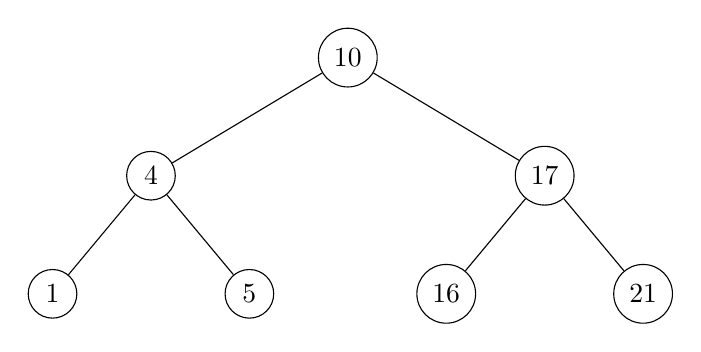
\begin{tikzpicture}[level/.style={sibling distance=50mm/#1}]
\node [circle,draw] (z){10}
  child {node [circle,draw] (a) {4}
    child {node [circle,draw] (b) {1}
      }
    child {node [circle,draw] (g) {5}
  }
  }
  child {node [circle,draw] (a) {17}
    child {node [circle,draw] (b) {16}
	}
    child {node [circle,draw] (g) {21}
  }
        };
\end{tikzpicture}

\begin{tikzpicture}[level/.style={sibling distance=50mm/#1}]
\node [circle,draw] (z){10}
  child {node [circle,draw] (a) {4}
    child {node [circle,draw] (b) {1}
      }
    child {node [circle,draw] (g) {5}
  }
  }
  child {node [circle,draw] (a) {16}
    child {node [circle,draw] (b) {17}
    child {node [circle,draw] (g) {21}
  }}
        };
\end{tikzpicture}

\begin{tikzpicture}[level/.style={sibling distance=50mm/#1}]
\node [circle,draw] (z){5}
  child {node [circle,draw] (a) {1}
    child {node [circle,draw] (g) {4}
  }
  }
  child {node[circle,draw] (y) {10}
  child {node [circle,draw] (a) {16}
    child {node [circle,draw] (b) {17}
    child {node [circle,draw] (g) {21}
  }}}
        };
\end{tikzpicture}

\begin{tikzpicture}[level/.style={sibling distance=50mm/#1}]
\node [circle,draw] (z){4}
  child {node [circle,draw] (a) {1}
  }
   child {node[circle,draw] (x) {5}
  child {node[circle,draw] (y) {10}
  child {node [circle,draw] (t) {16}
    child {node [circle,draw] (b) {17}
    child {node [circle,draw] (g) {21}
  }}}} };
\end{tikzpicture}

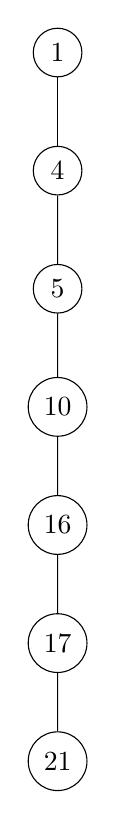
\begin{tikzpicture}[level/.style={sibling distance=50mm/#1}]
\node [circle,draw] (z){1}
  child {node [circle,draw] (x) {4}
   child {node[circle,draw] (t) {5}
  child {node[circle,draw] (y) {10}
  child {node [circle,draw] (a) {16}
    child {node [circle,draw] (b) {17}
    child {node [circle,draw] (g) {21}
  }}}}}
        };
\end{tikzpicture}

\noindent\textbf{Exercise 12.1-2}\\

The binary-search-tree property guarantees that all nodes in the left subtree are smaller, and all nodes in the right subtree are larger. The min-heap property only guarantees the general child-larger-than-parent relation, but doesn't distinguish between left and right children.  For this reason, the min-heap property can't be used to print out the keys in sorted order in linear time because we have no way of knowing which subtree contains the next smallest element. \\

\noindent\textbf{ Exercise 12.1-3} \\

Our solution to exercise 10.4-5 solves this problem.\\

\noindent\textbf{Exercise 12.1-4}\\

We call each algorithm on $T.root$. See algorithms PREORDER-TREE-WALK and POSTORDER-TREE-WALK.\\
\begin{algorithm}
\caption{PREORDER-TREE-WALK(x)}
\begin{algorithmic}
\If{$x \neq NIL$}
	\State print $x$
	\State PREORDER-TREE-WALK(x.left)
	\State PREORDER-TREE-WALK(x.right)
\EndIf
\State \textbf{return}
\end{algorithmic}
\end{algorithm}

\begin{algorithm}
\caption{POSTORDER-TREE-WALK(x)}
\begin{algorithmic}
\If{$x \neq NIL$}
	\State POSTORDER-TREE-WALK(x.left)
	\State POSTORDER-TREE-WALK(x.right)
	\State print $x$
\EndIf
\State \textbf{return}
\end{algorithmic}
\end{algorithm}


\noindent\textbf{ Exercise 12.1-5} \\


Suppose to a contradiction that we could build a BST in worst case time $o(n\lg(n))$. Then, to sort, we would just construct the BST and then read off the elements in an inorder traversal. This second step can be done in time $\Theta(n)$ by Theorem 12.1. Also, an inorder traversal must be in sorted order because the elements in the left subtree are all those that are smaller than the current element, and they all get printed out before the current element, and the elements of the right subtree are all those elements that are larger and they get printed out  after the current element. This would allow us to sort in time $o(n\lg(n))$ a contradiction\\


\noindent\textbf{ Exercise 12.2-1} \\

option $c$ could not be the sequence of nodes explored because we take the left child from the 911 node, and yet somehow manage to get to the 912 node which cannot belong the left subtree of 911 because it is greater. Option $e$ is also impossible because we take the right subtree on the 347 node and yet later come across the 299 node.\\

\noindent\textbf{Exercise 12.2-2}\\

See algorithms TREE-MINIMUM and TREE-MAXIMUM. \\

\begin{algorithm}
\caption{TREE-MINIMUM(x)}
\begin{algorithmic}
\If{$x.left \neq NIL$}
	\State \textbf{return} $TREE-MINIMUM(x.left)$
\Else
\State \textbf{return} $x$
\EndIf
\end{algorithmic}
\end{algorithm}

\begin{algorithm}
\caption{TREE-MAXIMUM(x)}
\begin{algorithmic}
\If{$x.right \neq NIL$}
	\State \textbf{return} $TREE-MAXIMUM(x.right)$
\Else
\State \textbf{return} $x$
\EndIf
\end{algorithmic}
\end{algorithm}

\noindent\textbf{ Exercise 12.2-3} \\

\begin{algorithm}
\caption{TREE-PREDECESSOR(x)}
\begin{algorithmic}
\If{$x.left \neq NIL$}
\State \Return TREE-MAXIMUM(x.left)
\EndIf
\State $y = x.p$
\While{$y\neq NIL$ and $x==y.left$}
\State $x=y$
\State $y=  y.p$
\EndWhile
\State\Return $y$
\end{algorithmic}
\end{algorithm}

\noindent\textbf{Exercise 12.2-4}\\

Suppose we search for 10 in this tree.  Then $A = \{9\}$, $B = \{8,10\}$ and $C = \emptyset$, and Professor Bunyan's claim fails since $8 < 9$.

\begin{tikzpicture}[level/.style={sibling distance=75mm/#1}]
\node [circle,draw] (a){8}
  child{ node [circle,draw] (e) {NIL}}
  child {
  node [circle,draw] (b) {10}
    child {node [circle,draw] (c) {9}
    }
      child {node [circle,draw] (d) {NIL}
      }
  };
\end{tikzpicture}

\noindent\textbf{ Exercise 12.2-5} \\

Suppose the node $x$ has two children. Then it's successor is the minimum element of the BST rooted at $x.right$. If it had a left child then it wouldn't be the minimum element. So, it must not have a left child. Similarly, the predecessor must be the maximum element of the left subtree, so cannot have a right child.\\

\noindent\textbf{Exercise 12.2-6}\\

First we establish that $y$ must be an ancestor of $x$.  If $y$ weren't an ancestor of $x$, then let $z$ denote the first common ancestor of $x$ and $y$.  By the binary-search-tree property, $x < z < y$, so $y$ cannot be the successor of $x$.  

Next observe that $y.left$ must be an ancestor of $x$ because if it weren't, then $y.right$ would be an ancestor of $x$, implying that $x > y$.  Finally, suppose that $y$ is not the lowest ancestor of $x$ whose left child is also an ancestor of $x$.  Let $z$ denote this lowest ancestor. Then $z$ must be in the left subtree of $y$, which implies $z < y$, contradicting the fact that $y$ is the successor if $x$. \\

\noindent\textbf{ Exercise 12.2-7} \\

To show this bound on the runtime, we will show that using this procedure, we traverse each edge twice. This will suffice because the number of edges in a tree is one less than the number of vertices.

Consider a vertex of a BST, say $x$. Then, we have that the edge between $x.p$ and $x$ gets used when successor is called on $x.p$ and gets used again when it is called on the largest element in the subtree rooted at $x$. Since these are the only two times that that edge can be used, apart from the initial finding of tree minimum. We have that the runtime is $O(n)$. We trivially get the runtime is $\Omega(n)$ because that is the size of the output.\\

\noindent\textbf{Exercise 12.2-8}\\

Let $x$ be the node on which we have called TREE-SUCCESSOR and $y$ be the $k^{th}$ successor of $x$. Let $z$ be the lowest common ancestor of $x$ and $y$. Successive calls will never traverse a single edge more than twice since TREE-SUCCESSOR acts like a tree traversal, so we will never examine a single vertex more than three times. Moreover, any vertex whose key value isn't between $x$ and $y$ will be examined at most once, and it will occur on a simple path from $x$ to $z$ or $y$ to $z$. Since the lengths of these paths are bounded by $h$, the running time can be bounded by $3k + 2h = O(k+h)$.\\


\noindent\textbf{ Exercise 12.2-9} \\

If $x = y.left$ then calling successor on $x$ will result in no iterations of the while loop, and so will return $y$. Similarly, if $x =y.right$, the while loop for calling predecessor(see exercise 3) will be run no times, and so $y$ will be returned. Then, it is just a matter of recognizing what the problem asks to show is exactly that y  is either predecessor(x) or successor(x).\\

\noindent\textbf{ Exercise 12.3-1} \\

The initial call to TREE-INSERT-REC should be NIL,T.root,z
\begin{algorithm}
\caption{TREE-INSERT-REC(y,x,z)}
\begin{algorithmic}
\If{$x \neq NIL$}
\If{$z.key < x.key$}
\State TREE-INSERT-REC(x,x.left,z)
\Else
\State TREE-INSERT-REC(x,x,right,z)
\EndIf
\EndIf
\State z.p = y
\If{$y==NIL$}
\State T.root = z
\ElsIf{$z.key <y.key$}
\State y.left = z
\Else
\State y.right = z
\EndIf
\end{algorithmic}
\end{algorithm}

\noindent\textbf{Exercise 12.3-2}\\

The nodes examined in the while loop of TREE-INSERT are the same as those examined in TREE-SEARCH.  In lines 9 through 13 of TREE-INSERT, only one additional node is examined. \\

\noindent\textbf{ Exercise 12.3-3} \\

The worst case is that the tree formed has height $n$ because we were inserting them in already sorted order. This will result in a runtime of $\Theta(n^2)$. In the best case, the tree formed is approximately balanced. This will mean that the height doesn't exceed $O(\lg(n))$. Note that it can't have a smaller height, because a complete binary tree of height $h$ only has $\Theta(2^h)$ elements. This will result in a rutime of $O(n\lg(n)$. We showed $\Omega(n\lg(n))$ in exercise 12.1-5.

\noindent\textbf{Exercise 12.3-4}\\

Deletion is not commutative.  In the following tree, deleting 1 then 2 yields a different from the one obtained by deleting 2 then 1.

\begin{tikzpicture}[level/.style={sibling distance=75mm/#1}]
\node [circle,draw] (a){2}
  child{ node [circle,draw] (e) {1}}
  child {
  node [circle,draw] (b) {4}
    child {node [circle,draw] (c) {3}
    }
      child {node [circle,draw] (d) {NIL}
      }
  };
\end{tikzpicture}

\noindent\textbf{ Exercise 12.3-5} \\

Our insertion procedure follows closely our solution to 12.3-1, the difference being that once it finds the position to insert the given node, it updates the succ fields appropriately instead of the p field of z.

\begin{algorithm}
\caption{TREE-INSERT'(y,x,z)}
\begin{algorithmic}
\If{$x \neq NIL$}
\If{$z.key < x.key$}
\State TREE-INSERT'(x,x.left,z)
\Else
\State TREE-INSERT'(x,x,right,z)
\EndIf
\EndIf
\If{$y==NIL$}
\State T.root = y
\ElsIf{$z.key <y.key$}
\State y.left = z
\State x.succ = y
\Else
\State y.right = z
\State z.succ = y.succ
\State y.succ = z
\EndIf
\end{algorithmic}
\end{algorithm}

Our Search procedure is unchanged from the version given in the previous section

We will assume for the deletion procedure that all the keys are distinct, as that has been a frequent assumption throughout this chapter. This will however depend on it. Our deletion procedure first calls search until we are one step away from the node we are looking for, that is, it calls TREE-PRED(T.root,z.key)

\begin{algorithm}
\caption{TREE-PRED(x,k)}
\begin{algorithmic}
\If{$k<x.key$}
\State $y = x.left$
\Else
\State $y = x.right$
\EndIf
\If{$y == NIL$}
\State throw error
\ElsIf{$y.key = k$}
\State \Return x
\Else
\State \Return TREE-PRED(y,k)
\EndIf
\end{algorithmic}
\end{algorithm}

It can use this TREE-PRED procedure to compute $u.p$ and $v.p$ in the TRANSPLANT procedure. Since TREE-DELETE only calls TRANSPLANT a constant number of times, increasing the runtime of TRANSPLANT to $O(h)$ in this way causes the runtime of the new TREE-DELETE procedure to be $O(h)$.\\

\noindent\textbf{Exercise 12.3-6}\\

Update line 5 so that $y$ is set equal to TREE-MAXIMUM(z.left). To implement the fair strategy, we could randomly decide each time TREE-DELETE is called whether or not to use the predecessor or successor. \\

\noindent\textbf{ Exercise 12.4-1} \\

Consider all the possible positions of the largest element of the subset of $n+3$ of size 4. Suppose it were in position $i+4$ for some $i\le n-1$. Then, we have that there are $i+3$ positions from which we can select the remaining three elements of the subset. Since every subset with different largest element is different, we get the total by just adding them all up (inclusion exclusion principle).\\

\noindent\textbf{Exercise 12.4-2}\\

To keep the average depth low but maximize height, the desired tree will be a complete binary search tree, but with a chain of length $c(n)$ hanging down from one of the leaf nodes. Let $k = \log(n-c(n))$ be the height of the complete binary search tree.  Then the average height is approximately given by 
\[ \frac{1}{n}\left[ \sum_{i=1}^{n - c(n)}\lg(i) + (k+1) + (k+2) + \ldots + (k+c(n))\right] \approx  \lg(n-c(n)) + \frac{c(n)^2}{2n}. \]

The upper bound is given by the largest $c(n)$ such that $\lg(n-c(n)) + \frac{c(n)^2}{2n} = \Theta(\lg n)$ and $c(n) = \omega(\lg n)$.  One function which works is $\sqrt{n}$.\\

\noindent\textbf{ Exercise 12.4-3} \\

Suppose we have the elements $\{1,2,3\}$. Then, if we construct a tree by a random ordering, then, we get trees which appear with probabilities some multiple of $\frac{1}{6}$. However, if we consider all the valid binary search trees on the key set of $\{1,2,3\}$. Then, we will have only five different possibilities. So, each will occur with probability $\frac{1}{5}$, which is a different probability distribution.\\

\noindent\textbf{Exercise 12.4-4}\\

The second derivative is $2^x \ln^2(2)$ which is always positive, so the function is convex. \\

\noindent\textbf{ Exercise 12.4-5} \\

Suppose that when quicksort always selects it's elements to be in the middle $n^{1-k/2}$ of the elements each time. Then, the size of the problem shrinks by a power of at least $(1-k/2)$ each time. So, the greatest depth of recursion $d$ will be so that $n^{(1-k/2)^d} \le2$, solving for $d$, we get $(1-k/2)^d \le \log_n(2) = \lg(2)/\lg(n)$, so, $d \le \log_{1-k/2}(\lg(2)) - \log_{1-k/2}(\lg(n) = \log_{1-k/2}(\lg(2)) - \lg(\lg(n))/ \lg(1-k/2)$.

Let A(n) denote the probability that when quicksorting a list of length $n$, some pivot is selected to not be in  the middle $n^{1-k/2}$ of the numbers. This doesn't happen with probability $\frac{1}{n^{k/2}}$. Then, we have that the two subproblems are of size$n_1,n_2$ with $n_1+n_2 = n-1$ and $\max\{n_1,n_2\} \le n^{1-k/2}$. So, $A(n) \le \frac{1}{n^{k/2}} + T(n_1)+T(n_2)$ So, since we bounded the depth by $O(1/\lg(n))$ let $\{a_{i,j}\}_i$ be all the subproblem sizes left at depth $j$. So, $A(n) \le \frac{1}{n^{k/2}}\sum_{j} \sum_i \frac{1}{a}$

\noindent\textbf{Problem 12-1} \\

\begin{enumerate}[a.]
\item
Each insertion will add the element to the right of the rightmost leaf because the inequality on line 11 will always evaluate to false. This will result in the runtime being $\sum_{i=1}^n i \in \Theta(n^2)$

\item
This strategy will result in each of the two children subtrees having a difference in size at most one. This means that the height will be $\Theta(\lg(n))$. So, the total runtime will be $\sum_{i=1}^n \lg(n) \in \Theta(n\lg(n))$

\item
This will only take linear time since the tree itself will be height 0, and a single insertion into a list can be done in constant time.

\item
The worst case performance is that every random choice is to the right (or all to the left) this will result in the same behavior as in the first part of this problem, $\Theta(n^2)$

To compute the expected runtime informally, just notice that when randomly choosing, we will pick left roughly half the time, so, the tree will be roughly balanced, so, we have that the depth is roughly $\lg(n)$, so the expected runtime will be $n\lg(n)$.


\end{enumerate}

\noindent\textbf{Problem 12-2}\\

The word at the root of the tree is necessarily before any word in its left or right subtree because it is both shorter, and the prefix of, every word in each of these trees.  Moreover, every word in the left subtree comes before every word in the right subtree, so we need only perform a preorder traversal.  This can be done recursively, as shown in exercise 12.1-4. \\


\noindent\textbf{Problem 12-3} \\

\begin{enumerate}[a.]
\item
Since we are averaging over all nodes $x$ the value of $d(x,T)$, it is $\frac{1}{n} \sum_{x\in T} d(x,T)$, but by definition, this is $\frac{1}{n} P(T)$.

\item
Every non-root node has a contribution of one coming from the first edge from the root on its way to that node, every other edge in this path is counted by looking at the edges within the two subtrees rooted at the child of the original root. Since there are $n-1$ non-root nodes, we have
\[
P(T) = \sum_{x\in T} d(x,T) = \sum_{x\in T_L} d(x,T) + \sum_{x\in T_R} d(x,T) =\]\[ \sum_{x\in T_L} (d(x,T_L)+1) + \sum_{x\in T_R}(d(x,T_R)+1) = \sum_{x\in T_L}d(x,T_L) + \sum_{x\in T_R}d(x,T_R) + n-1 =\]\[ P(T_L) + P(T_R) +n-1
\]

\item
When we are randomly building our tree on n keys, we have $n$ possibilities for the first element that we add to the tree, the key that will belong to the eventual root. Suppose that it had order statistic $i+1$ for some $i$ in $\{0,\ldots  n-1\}$. Then, we have that all the smaller elements will be to the left and all the larger elements will be in the subree to the right. However, they will all be in random order relative to each other, so, we will have $P(i) = E[P(T_L)]$ and $P(n-i-1) = E[P(T_R)]$. So, we have have the desired inequality by averaging over the order statistic of the first term put into the BST.

\item
\[
\frac{1}{n} \sum_{i=0}^{n-1} P(i) + P(n-i-1) + n-1 = \frac{1}{n}\left(\sum_{i=0}^{n-1}P(i) + \sum_{i=0}^{n-1}P(n-i-1) + \sum_{i=0}^{n-1}(n-1)\right)
\]

Then, we do the substitution $j = n-i-1$ and do the simple thing of summing a constant for the third sum to get

\[
=  \frac{1}{n}\left(\sum_{i=0}^{n-1}P(i) + \sum_{j=0}^{n-1}P(j) + n(n-1)\right) = \frac{2}{n} \sum_{i=0}^{n-1} P(i) + n-1
\]

\item
Our recurrence from the previous part is exactly the same as eq (7.6) which we showed in problem 7-3.e to have solution $\Theta(n\lg(n))$

\item
Let the first pivot selected be the first element added to the binary tree. Since every element is compared to the root, and every element is compared to the first pivot, we have what we want. Then, let the next pivot for the left (resp. right) subarrays be the first element that is less than (resp. greater than) the root. Then, we have that the two subtrees form the same partition of the remaining elements as the two subarrays left form. We can than continue to recurse in this way. Since if holds at the first element, and the problems have the same recursive structure, we have that it holds at every element.

\end{enumerate}

\noindent\textbf{Problem 12-4}\\
\begin{enumerate}[a.]
\item There is a single binary tree on one vertex consisting of just a root, so $b_0 = 1$.  To count the number of binary trees with $n$ nodes, we first choose a root from among the $n$ vertices.  If the root node we have chosen is the $i^{th}$ smallest element, the left subtree will have $i-1$ vertices, and the right subtree will have $n-i$ vertices.  The number of such left and right subtrees are counted by $b_{i-1}$ and $b_{n-i}$ respectively.  Summing over all possibly choices of root vertex gives:

\[ b_n = \sum_{k=1}^n b_{k-1}b_{n-k} = \sum_{k=0}^{n-1} b_kb_{n-k-1}.\]

\item

\begin{align*}
B(x) &= \sum_{n=0}^\infty b_nx^n \\
&= 1 + \sum_{n=1}^\infty b_nx^n \\
&= 1+ \sum_{n=1}^\infty  \sum_{k=0}^{n-1} b_kb_{n-k-1} x^n \\
&= 1+ x\sum_{n=1}^\infty  \sum_{k=0}^{n-1} b_kx^kb_{n-k-1} x^{n-k-1} \\
&= 1+ x\sum_{n=0}^\infty  \sum_{k=0}^{n} b_kx^kb_{n-k} x^{n-k} \\
&= 1 + xB(x)^2.
\end{align*}
Applying the quadratic formula and noting that the minus sign is to be taken so that $B(0) = 0$ proves the result. \\

\item Using the Taylor expansion of $\sqrt{1-4x}$ we have:
\begin{align*}
B(x) &= \frac{1}{2x}\left(1-\sum_{n=0}^\infty \frac{1}{1-2n}{2n \choose n}x^n\right) \\
&=\frac{-1}{2x}\sum_{n=1}^\infty \frac{1}{1-2n}{2n \choose n}x^n \\
&= \frac{1}{2}\sum_{n=1}^\infty \frac{1}{2n-1}{2n \choose n}x^{n-1} \\
&=\frac{1}{2}\sum_{n=0}^\infty \frac{1}{2n+1}{2n+2 \choose n+1}x^{n}. \\
\end{align*}
Extracting the coefficient from $x^n$ and simplifying yields the result. \\

\item The asymptotic follows from applying Sirling's formula to $b_n$.

\end{enumerate}


\end{document} 